\documentclass[11pt]{article}
\usepackage[margin=1in]{geometry}
\usepackage{amsmath,amssymb}
\usepackage[T1]{fontenc}
\usepackage[utf8]{inputenc}
\usepackage{booktabs}
\usepackage{verbatim}
\usepackage{graphicx}
\usepackage{placeins}
\graphicspath{{../figures/}{../../figures/}}

\title{Bitter solenoid simulator:\\continuum model, mesoscopic emulation, and the living record}
\author{s-siyanwal/bitter-solenoid-simulator}
\date{\today}

\begin{document}
\maketitle

\begin{abstract}
This note records the physics, the algorithms, and the numbers of the 0.5~T water-cooled copper Bitter-solenoid simulator.
The continuum solver is the reference.
The mesoscopic emulation is a separate layer.
It is not molecular dynamics, and it is not a particle model of the roughly 2575~kg winding.
Section~\ref{sec:measured} compares the bare solver with measurements on five built magnets, adds explicit layer stacks with a PEEC AC-impedance model, and records what does and does not generalize.
Tables in the generated section are rewritten by \texttt{examples/update\_report.py} after \texttt{examples/run\_all.py} or \texttt{examples/run\_emulation.py}.
A code or results change appends the changelog in the same commit.
\end{abstract}

\section{What the two layers are}

The continuum package evaluates one design: geometry, current locked to a target on-axis field, copper temperature, channel flow, thin-ring hoop stress, and a Swiss-roll radiofrequency coating whose static permeability is exactly 1.
The optimiser searches that map.

The emulation layer does not replace that evaluation.
It reports a Drude representative volume at the inner radius, a seeded Langevin cloud inside that volume, Johnson noise on the supply sense, and a Monte Carlo of manufacturing and contact scatter around the same continuum call.
Every emulation object carries the label ``mesoscopic emulation, not molecular dynamics''.

Model grades, written into the JSON:
\begin{itemize}
\item established: Drude identities, Johnson--Nyquist, shot-versus-Johnson comparison, Antoine saturation temperature;
\item approximate: Kohler magnetoresistance with a coefficient of order 1, the Langevin picture, log-normal contact resistance, tolerances, Bergles--Rohsenow onset of nucleate boiling, housing convection, the optional radial resistivity note;
\item speculative: Hooge-like $1/f$ (default off) and the Swiss-roll signal-to-noise gain.
\end{itemize}

\section{Continuum field}

Amp\`ere's law for a long thin solenoid is $B=\mu_0 n I$.
A finite thin solenoid is $B_z(0)=\frac12\mu_0 n I(\cos\theta_1+\cos\theta_2)$.
A thick winding with uniform current density has the logarithmic closed form.
A Bitter plate has $J_\phi = C/r$ because the resistive sheet between two radii is a solution of Laplace's equation for the voltage.
On axis,
\begin{equation}
B_z(0)=\mu_0 C\left[\operatorname{asinh}\frac{L}{2R_1}-\operatorname{asinh}\frac{L}{2R_2}\right].
\end{equation}
Off axis the winding is a set of Gauss--Legendre coaxial loops.
Each loop uses the complete elliptic integrals $K(m)$ and $E(m)$, evaluated with the arithmetic-geometric mean so the browser and the Numba kernel share the same limit.
The straight-segment Biot--Savart engine is an independent check, not the design loop.
Homogeneity is the peak-to-peak spread of $|B|$ on a 30~mm diameter spherical volume, in parts per million of the isocentre field.
The current is chosen so the closed-form centre field equals the requested $B_0$, usually 0.5~T.
The loop model then reports a numerical centre field that agrees with that lock to well under a microtesla on the published designs.

Fill. Insulation thickness $d_i$ and the hole area fraction $f_h$ reduce the copper:
\begin{equation}
\lambda = \frac{d}{d+d_i}(1-f_h),\qquad
N = \frac{L}{d+d_i},\qquad
I = \frac{C L \ln(R_2/R_1)}{N}.
\end{equation}
Electrical power at the mean copper temperature, with resistivity $\rho(T)=\rho_{20}[1+\alpha(T-20)]$, is
\begin{equation}
P = \frac{2\pi \rho(T)\, C^2 L \ln(R_2/R_1)}{\lambda}.
\end{equation}
The published optimum uses a uniform $\rho(T)$.
An optional radial correction is reported and left off, so those numbers stay put.

\section{Heat and water}

Bulk water properties are the same correlations in Python and in \texttt{docs/bittersim.js}.
A channel of diameter $D$ and speed $v$ has Reynolds and Prandtl numbers from those properties.
Turbulent Nusselt numbers are Dittus--Boelter, $0.023\,\mathrm{Re}^{0.8}\mathrm{Pr}^{0.4}$, and Gnielinski.
Laminar channels use $\mathrm{Nu}=4.36$.
Darcy friction is $64/\mathrm{Re}$ below 2300 and the Petukhov smooth-pipe formula above it.
Pressure drop adds a minor-loss coefficient of 1.5.
Pump shaft power divides hydraulic power by $\eta=0.7$.

The stack is iterated at fixed current constant $C$: update power, mixed-cup temperature rise $P/(\dot m c_p)$, film drop, and mean copper temperature until the increment is below $10^{-10}$~K.
The hot spot is the inner hole row at the outlet.
That channel carries only its own heat.
Conduction through the plate to the hole is an annular fin with an insulated outer boundary,
\begin{equation}
\Delta T_{\mathrm{cond}} = \frac{q}{4k}\left[2b^2\ln\frac{b}{a}-(b^2-a^2)\right].
\end{equation}
The lumped transient is one copper node and quasi-steady water.
With cooling removed, temperature runs away adiabatically.
On the seed-1 optimum that integrator reaches 85~C in 4922~s.
That figure is not a boiling model.
The emulation flags the adiabatic curve at the Antoine saturation temperature and stops interpreting it there.
On the PDF initial guess that saturation time is about 479~s.
The two captions must not be swapped.

Antoine, for site pressure in bar inside about 0.7 to 2~bar,
\begin{equation}
T_{\mathrm{sat}}/^\circ\mathrm{C} = \frac{1730.63}{5.1962-\log_{10}(p/\mathrm{bar})}-233.426.
\end{equation}
At 101325~Pa this is 100~C within half a degree.
Onset of nucleate boiling, water only, is Bergles--Rohsenow (1964).
Other catalog coolants do not inherit that water formula.
The mixed outlet is asked to stay 10~K under saturation.
There is no critical-heat-flux map.

\section{Mechanics and the Swiss roll}

The thin-ring hoop bound is $\sigma = C B_0/\lambda$.
A field-profile integral gives a slightly smaller stress.
Both are about 0.12~MPa on the optimum, far under hard-copper yield.
The 0.5~T design is not stress-limited.
Axial force compresses each half of the stack.
Round graded holes are not a Florida-Bitter plate: real plates use elongated staggered holes because round holes crowd current.

The Swiss roll is a Pendry--Lorentzian coating,
\begin{equation}
\mu_{\mathrm{eff}}(\omega)=1-\frac{F\omega^2}{\omega^2-\omega_0^2+i\omega\Gamma},
\end{equation}
with geometric $\omega_0$, skin-effect sheet resistance, and a loss multiplier that puts $Q$ near 97.
At zero frequency, $\mu_{\mathrm{eff}}=1$, so the roll does not move $B_0$ or the homogeneity in this model.
The signal-to-noise expression is a heuristic (reciprocity, a flux guide, and a $\mu''$ noise term).
It is not an MRI measurement.

\section{Optimiser}

Decision variables are inner radius, build $(R_2-R_1)$, length, plate thickness, hole diameter, water speed, and pitch ratio.
Voltage is derived.
The objective is electrical power plus pump shaft power.
Inequality limits, written as $g\ge 0$ inside the code, are hot spot $\le 85~^\circ$C, supply $\le 8$~V, homogeneity $\le 100$~ppm, pressure drop $\le 5$~bar, $\mathrm{Re}\ge 10^4$, and $R_2\le 0.3$~m, together with the box bounds in \texttt{optimize.py}.

\begin{verbatim}
procedure OPTIMISE(seed, bounds, limits):
    population <- differential_evolution(objective, bounds, seed)
    best <- member with smallest P_elec + P_pump among feasible members
    polished <- SLSQP(best) with finite-difference gradients
    return polished if it improves the objective and stays feasible
           else best
end procedure
\end{verbatim}

The published seed-1 run used 10605 evaluations.
SLSQP did not improve it.
Active limits were homogeneity, both radii, Reynolds number, and plate and pitch near their upper bounds.
Hot-spot temperature and voltage had a large margin.
This report does not replace that table when the same code is re-run on another machine.
A changed algorithm would be a new row, with its own seed and version.

\section{Catalog}

Only listed identifiers are legal.
An unknown id raises \texttt{ValueError} and prints the list.
Conductors: OFHC copper (default), a Cu--Ag approximation, a Cu--Zr approximation, and aluminium 1350, which is allowed with a warning and is not recommended.
Coolants, liquid only: deionized water (the existing correlations), 30~percent water--glycol (conductive, not a dielectric), and a Galden HT135-class fluorocarbon (dielectric, lower heat-transfer coefficient).
The continuum JavaScript core still uses water correlations; the page says so when Galden is selected.
Insulators: polyimide, mica, PTFE, G-10.
G-10 between wet plates warns.
Housing (304 stainless, G-10 bore, 6061 aluminium) adds an external-convection estimate at $8~\mathrm{W\,m^{-2}K^{-1}}$ and a mass.
It is not subtracted from the copper power.
A conductive bore is a warning, not an eddy-current finite-element solution.
No FEniCS model is included.

\section{Mesoscopic emulation}

Constants shared with the browser, so the identities match to $10^{-9}$:
$e=1.60217662\times 10^{-19}~\mathrm{C}$,
$m_e=9.1093837\times 10^{-31}~\mathrm{kg}$,
$k_B=1.38064852\times 10^{-23}~\mathrm{J\,K^{-1}}$.

Drude, at the inner-radius copper:
\begin{align}
\rho &= \frac{m_e}{n e^2 \tau},&
v_d &= \frac{J}{n e},&
\lambda &= v_F \tau,\\
\omega_c\tau &= \frac{eB}{m_e}\tau,&
\frac{\Delta\rho}{\rho} &= a(\omega_c\tau)^2.
\end{align}
The Kohler coefficient $a$ defaults to 1 and defaults to on only inside the emulation.
With Kohler off, $\mathbf{J}\cdot\mathbf{E}=\rho J^2$ exactly.
At 0.5~T the Hall angle is far below $10^{-2}$, so magnetoresistance is negligible for this magnet.
Drift is about $10^{-3}~\mathrm{m\,s^{-1}}$ or less.
The mean free path is tens of nanometres.

The Langevin step is one-dimensional and lives only in that volume.
NumPy's \texttt{RandomState} is used so the picture does not depend on the Generator API.
\begin{equation}
\mathrm{d}v = -\frac{v}{\tau}\mathrm{d}t + \frac{v_d}{\tau}\mathrm{d}t
+ \sqrt{\frac{2k_B T}{m_e\tau}}\,\mathrm{d}W,
\qquad \mathrm{d}t=\tau/20.
\end{equation}
At room temperature the thermal speed dwarfs $v_d$, so a few dozen carriers do not resolve the drift.
A zero-temperature test must converge to $v_d$.
The cloud on the web page is the same formula with an independent mulberry32 stream.
It is not a drawing of $10^{28}$ carriers.

Johnson voltage spectral density is $S_V=4k_B T R$, integrated from 1~Hz to 10~kHz by default.
A 1~Hz bin at the Larmor frequency is a density, not the MRI noise floor.
Shot noise $\sqrt{2e I\,\mathrm{d}f}$ is negligible next to Johnson current noise in this metal.
Hooge $1/f$ is off unless requested, and the browser does not apply it.

Monte Carlo, seed required.
The reference sample is Python, default 200 draws.
The verified comparison used 50 draws and seed 1.
Scatter, all labeled as assumptions: radii normal with $\sigma=0.2$~mm, length $\sigma=0.5$~mm, hole and plate uniform $\pm 1$~percent, inlet temperature $\sigma=0.2$~K, inner-row speed uniform $\pm 10$~percent, resistivity lot uniform $\pm 2$~percent, contact resistance log-normal with median $10^{-6}~\Omega$ per interface and $\sigma_{\ln}=1$.
The number of interfaces is $\max(1,\mathrm{round}(N)-1)$.
Supply current is the nominal value.
$B_0$ is recomputed from that current and the perturbed turns and radii, then \texttt{evaluate\_design} is called so the lock matches a fixed-current field.
Contact scales voltage, power, and the temperature rise by $(R+R_c)/R$.
The lot multiplies resistivity inside the evaluator.
Percentiles are 5, 50 and 95.
Bias is the median minus the nominal continuum value.
Trip fractions: hot spot above 85~C, ONB margin below 0, hoop stress above 0.6 times the selected temper yield.

\begin{verbatim}
procedure EMULATE(design, n, seed, catalog):
    nominal <- EVALUATE(design, catalog)
    rng <- RandomState(seed)
    for i in 1..n:
        q <- perturb geometry, flow, inlet, resistivity lot
        Rc <- sum of log-normal contact draws
        q.B0 <- field of the nominal current in the perturbed geometry
        sample <- EVALUATE(q)
        scale <- (R_sample + Rc) / R_sample * lot
        record B0, V*scale, P*scale, T scaled the same way,
               drift, mean free path, Johnson voltage
    return percentiles, trip fractions, warnings, model_grade
end procedure
\end{verbatim}

The browser subset caps $n$ at 300, skips the loop homogeneity inside each draw, and uses a different random stream.
Its ppm column is the continuum value.
Python is the reference when the two disagree.

% Measured-data validation, October 2026. Included from bitter_solenoid_report.tex.
\section{Validation against measured magnets (October 2026)}
\label{sec:measured}

The sections above verify the solver against closed forms.
This section compares the \emph{bare} solver with measurements on built magnets.
No parameter is fitted to a measurement.
Two campaigns, Olsen Bitter-ZS and Claw-ZS, are held out of every training set of the residual corrector; their rows are scores of physics changes, not fits.
Convention: relative residual $=(\text{measured}-\text{solver})/\text{solver}$, flagged when its magnitude exceeds 5\,\%.
Everything here is reproduced by \texttt{tests/test\_arxiv\_checks.py}, \texttt{tests/test\_stack.py}, \texttt{examples/generalization\_table.py}, \texttt{examples/joint\_diagnostic.py} and \texttt{examples/make\_arxiv\_figures.py}.

\subsection{New closed-form checks from the papers}
\begin{itemize}
\item \textbf{Thin Bitter arc (Sabulsky et al., arXiv:1309.5330, Eq.~6).} For a plate of thickness $t\to0$ with $Ct$ fixed, E4 tends to
$B_z(z)=\tfrac{\mu_0 Ct}{2}\left[(a_1^2+z^2)^{-1/2}-(a_2^2+z^2)^{-1/2}\right]$.
The code reaches $10^{-8}$ at $t=10\,\mu$m, the error falls as $t^2$, and Eq.~6 equals a 64-node radial loop integral to $10^{-10}$.
\item \textbf{Long stack (Kobelev, arXiv:1610.06607, Eq.~2.6).} $B_0\to\mu_0C\ln(R_2/R_1)$ as $L\to\infty$ with an $O((R/L)^2)$ end correction, and the in-winding field used for the hoop stress tends to $\mu_0C\ln(R_2/r)$ (0.21\,\% of $B_0$ at $L=4$~m).
\end{itemize}

\subsection{Explicit layer stacks}
Built magnets are tables of plates, half-plates, brass end pieces and spacers.
\texttt{bittersim/stack.py} keeps each layer: E4 ($J=C/r$) or E3 (uniform) per layer, weighted by the arc fraction $\varphi/2\pi$, mirrored pairs with either current sign, and per-layer DC resistance
\begin{equation}
R_{\text{layer}}=\frac{\rho\,\varphi}{t\ln(R_2/R_1)}\quad(J=C/r),\qquad
R_{\text{total}}=\sum R_{\text{layer}} + n_j r_j + R_{\text{leads}},
\end{equation}
with $r_j=R_{\text{leads}}=0$ unless a measured value is supplied.
The DC inductance splits each layer into $n_r\times n_z$ filaments, $L=\sum_{ij}w_iw_jM_{ij}$ with the Maxwell mutual (E8) and a rectangular-ring self term $\mu_0r[\ln(8r/g)-2]$, $g=0.2235(\Delta r+\Delta z)$.
It reproduces E9 to 0.5\,\% on a flat spiral and on a 40-plate stack.

\paragraph{AC impedance (PEEC).}
The filaments of one layer are in parallel and the layers are in series:
\begin{equation}
(\mathbf R_f + j\omega\mathbf M)\,\mathbf i=\mathbf P\,\mathbf V,\qquad \mathbf P^{\mathsf T}\mathbf i=\mathbf s,\qquad Z(\omega)=\mathbf s^{\mathsf T}\mathbf V,
\end{equation}
where $\mathbf s$ holds the layer currents ($\pm1$, or $\tfrac12$ for a smeared half-turn).
At $\omega\to0$ this returns $J=C/r$, the plate resistance and the DC inductance exactly.
At AC the current crowds toward the bore once the skin depth approaches the \emph{radial width} of the plate (not its thickness), so the apparent inductance falls and the resistance rises.

\subsection{Data used}
\begin{center}\small
\begin{tabular}{@{}llll@{}}
\toprule
magnet & measured target & geometry source & split \\
\midrule
EPFL bulk-machined spiral (arXiv:1901.08791) & Hall point, $R$, $L$ & paper Sec.~2 & published bench\\
Claw-ZS (arXiv:2607.02813) & $B_z(z)$, $R$, $Z(f)$ with phase & \texttt{CZS\_radia.py} & held out\\
JQI Bitter Ioffe--Pritchard (arXiv:2008.11181) & $B_0$, $B'$, $B''$, $R$, $L$ & design notebook & published bench\\
Olsen Bitter-ZS (arXiv:2510.21064) & $|Z(f)|$, $R$ & locked A\_358 table & held out\\
RRE 441~mm stripwound (1972) & 50~kG at 17\,275~A & paper (gap missing) & bound only\\
\bottomrule
\end{tabular}\end{center}

\subsection{Field}
Where the winding geometry is known the field closes: the EPFL Hall point is $-0.3$\,\% (1.2835 vs 1.28~G/A), the Claw-ZS peak is $-1.1$\,\% and its 46-point profile has an RMS residual of 0.100~mT (Fig.~\ref{fig:clawbz}).
For JQI the \emph{shape} closes ($B''/B_0$ within 0.1\,\%, $B'/B_0$ within 2.8\,\%) while the amplitude is 9--12\,\% high on all four coefficients (Fig.~\ref{fig:jqi}); the same layer table reproduces the authors' own resistance estimates, so the as-built turn count is the open question, not the field law.

\begin{figure}[ht]\centering
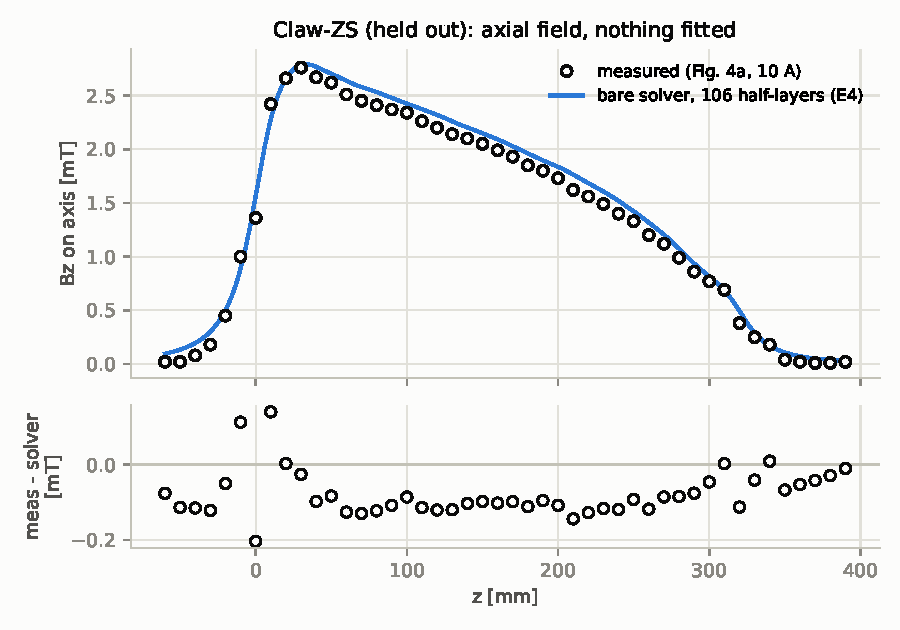
\includegraphics[width=0.78\textwidth]{fig14_clawzs_bz}
\caption{Claw-ZS axial field at 10~A: digitised measurement (Fig.~4a of the paper) against the bare solver built from the deposited layer table. Nothing fitted.}
\label{fig:clawbz}
\end{figure}

\begin{figure}[ht]\centering
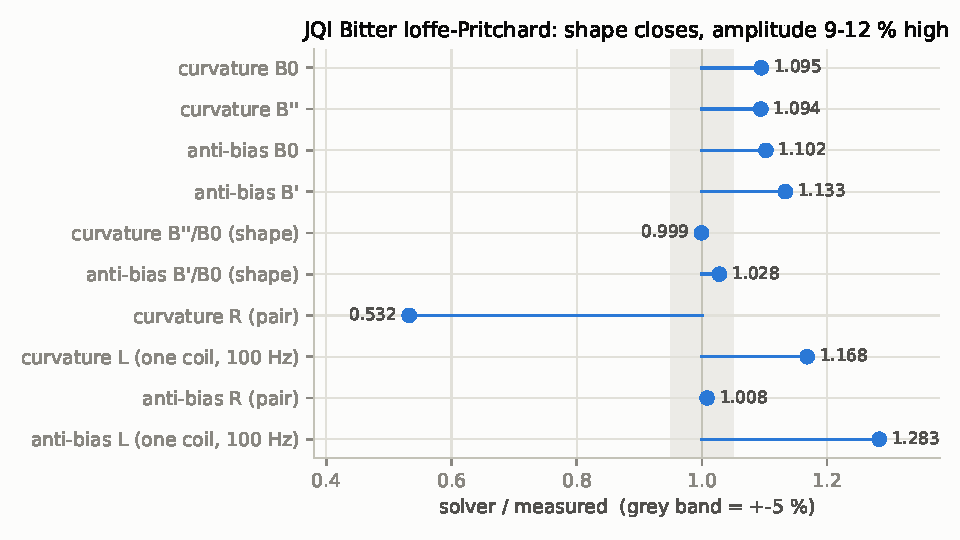
\includegraphics[width=0.82\textwidth]{fig15_jqi_ratios}
\caption{JQI coils: solver/measured for field coefficients, shape ratios, resistance and inductance (grey band $\pm5$\,\%).}
\label{fig:jqi}
\end{figure}

\subsection{Inductance is an AC quantity}
The earlier comparisons put the DC geometric inductance 57\,\% (Claw-ZS) and 79\,\% (Olsen) above the published values.
The PEEC model shows why: the published values are kHz-dominated.
With nothing fitted, Claw-ZS $L(f)$ closes within 3\,\% from 20~Hz to 2~kHz and the impedance phase within 3$^\circ$, against up to 11$^\circ$ for the DC model (Fig.~\ref{fig:claw}).
For Olsen, whose deposited data is $|Z|$ only, the 10~kHz miss falls from $+81$\,\% to $+23$\,\% (Fig.~\ref{fig:olsen}); the remainder is consistent with the Cu spacer sector, slit and holes that the axisymmetric stack omits, and a steady $+6$\,\% low-frequency offset is the $|Z|$ scale (24.9 vs 26.5~m$\Omega$).
The absolute Claw-ZS match holds only under the $\times10$ reading of the deposited impedance scale, which it therefore supports.

\begin{figure}[ht]\centering
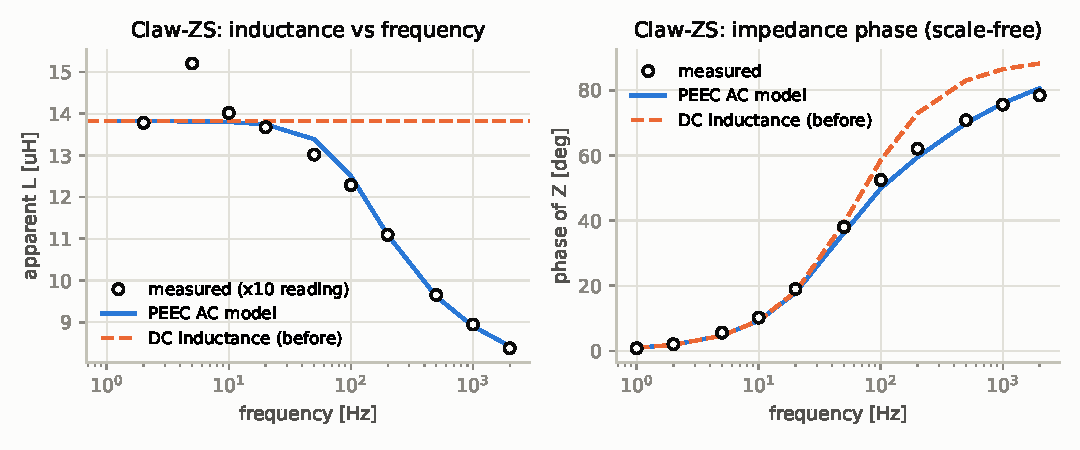
\includegraphics[width=\textwidth]{fig12_clawzs_impedance}
\caption{Claw-ZS (held out): apparent inductance and impedance phase against frequency. Black: lock-in reduction of the deposited traces. Blue: PEEC AC model. Orange dashed: DC inductance.}
\label{fig:claw}
\end{figure}

\begin{figure}[ht]\centering
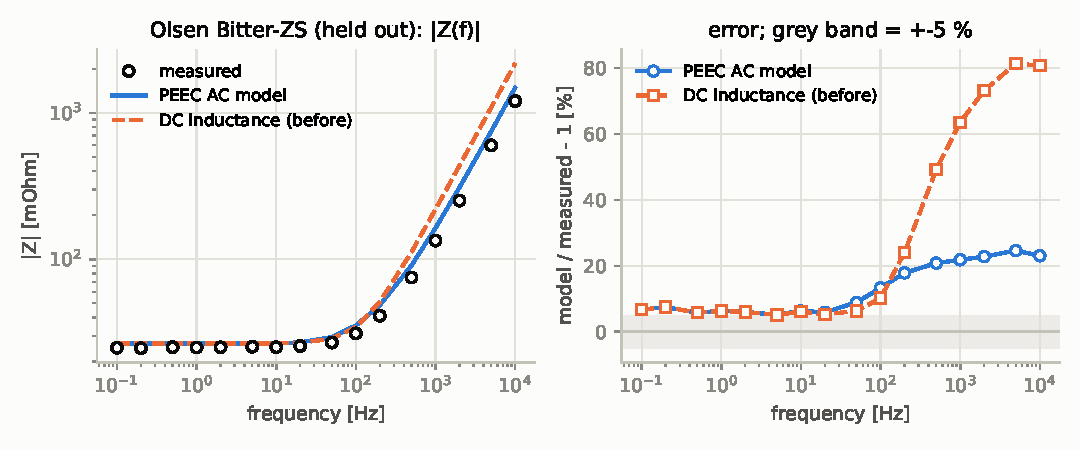
\includegraphics[width=\textwidth]{fig13_olsen_impedance}
\caption{Olsen Bitter-ZS (held out): $|Z(f)|$ and model error. Only the measured DC resistance enters, as a frequency-independent contact term. The steady $+6$\,\% offset below 100~Hz is the $|Z|$ scale of the deposited data (24.9 vs 26.5~m$\Omega$).}
\label{fig:olsen}
\end{figure}

\subsection{Resistance does not generalize}
The layer model is low on every coil except the JQI anti-bias pair ($-0.8$\,\%): EPFL $+24$\,\%, Claw-ZS $+45$\,\%, JQI curvature $+88$\,\%, Olsen $\times4.8$ (a faulty contact reported by the authors).
If joints carried the gap, the per-interface values would agree; they do not (Fig.~\ref{fig:joint}): 7.8(1.0)~$\mu\Omega$ for Claw-ZS, 215(30) and $-5(41)$~$\mu\Omega$ for two JQI coils of the same construction, and the EPFL spiral has a 2~m$\Omega$ gap with no joints at all.
The extra resistance is coil- and set-up-specific (leads, terminals, voltage taps), so the model keeps $r_j=R_{\text{leads}}=0$ and $R$ is not a corrector target.

\begin{figure}[ht]\centering
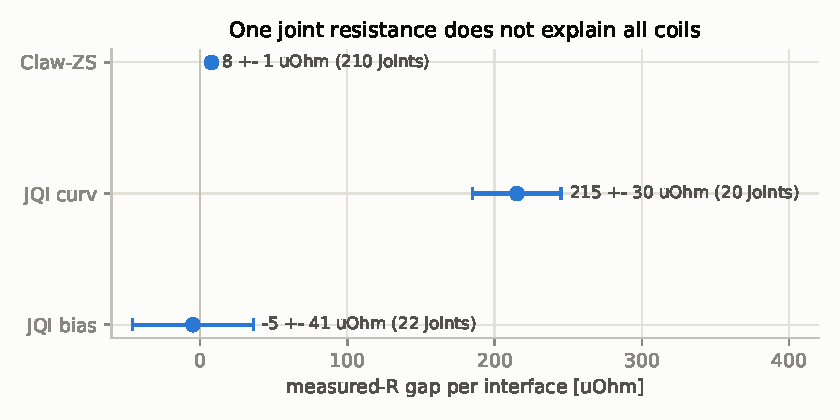
\includegraphics[width=0.7\textwidth]{fig17_joint_diagnostic}
\caption{Measured-resistance gap divided by the number of current-carrying interfaces.}
\label{fig:joint}
\end{figure}

\subsection{Scorecard and a 1972 bound}
Fig.~\ref{fig:score} collects every row (\texttt{results/GENERALIZATION.md}).
The 1972 RRE paper gives a 441~mm-bore stripwound solenoid (16 pancakes $\times$ 15 turns of two paralleled $43\times8$~mm strips, 17\,275~A, ``50~kG''), but not the gap between pancakes.
E3 gives 5.41~T at zero gap and 5.11~T at 5~mm (Fig.~\ref{fig:rre}); copper-only $R$ is 12.5--14.5~m$\Omega$ (20--60~$^\circ$C) against 280~V/17\,275~A $=16.2$~m$\Omega$.
It is consistent, and it is a bound, not a validation.
The companion 1972 IRD paper (Mulhall) gives design scaling and ``just over 18~T at 4.75~MW'' in a 28~mm bore with no coil table.

\begin{figure}[ht]\centering
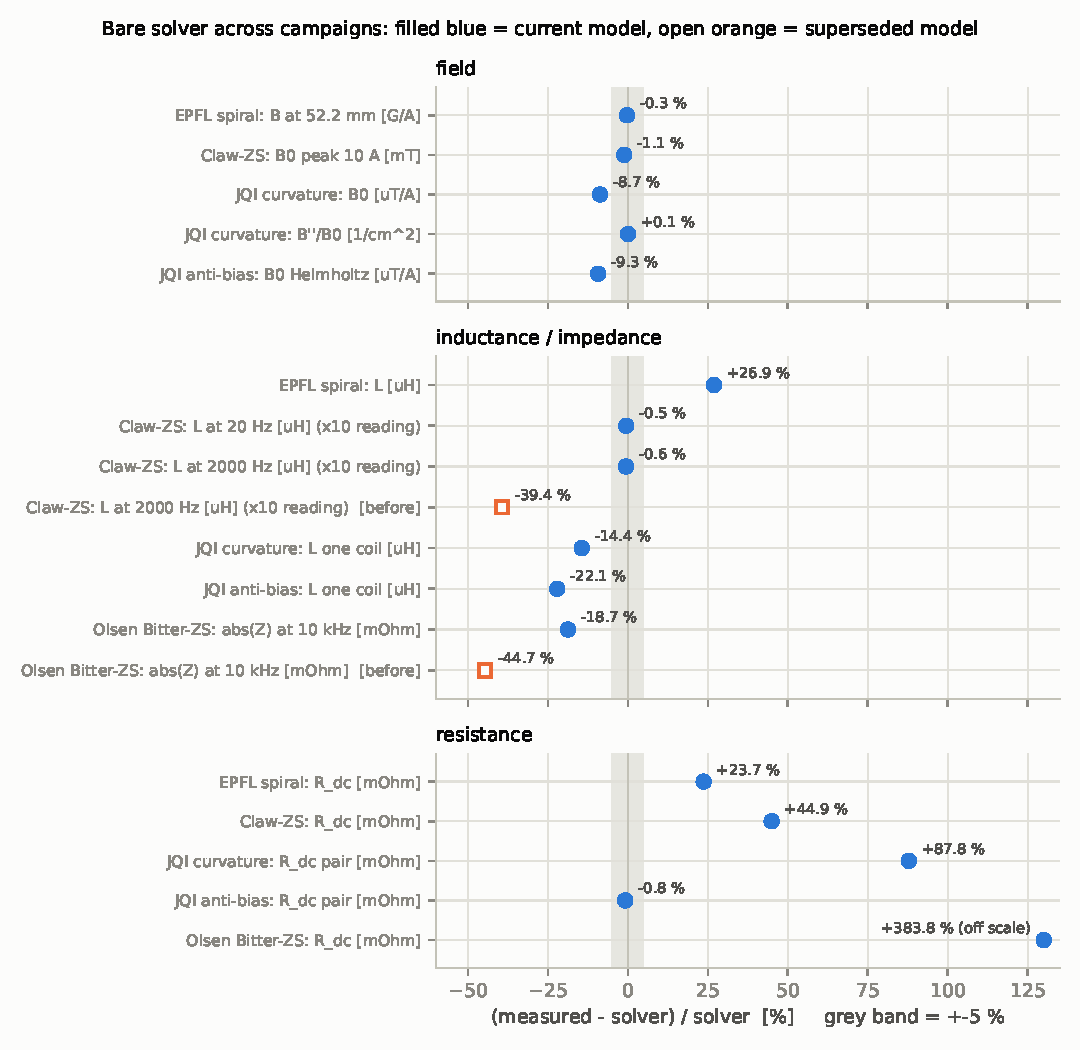
\includegraphics[width=0.86\textwidth]{fig16_scorecard}
\caption{Bare-solver residuals by campaign and channel. Filled blue: current model. Open orange: superseded DC-inductance model.}
\label{fig:score}
\end{figure}

\begin{figure}[ht]\centering
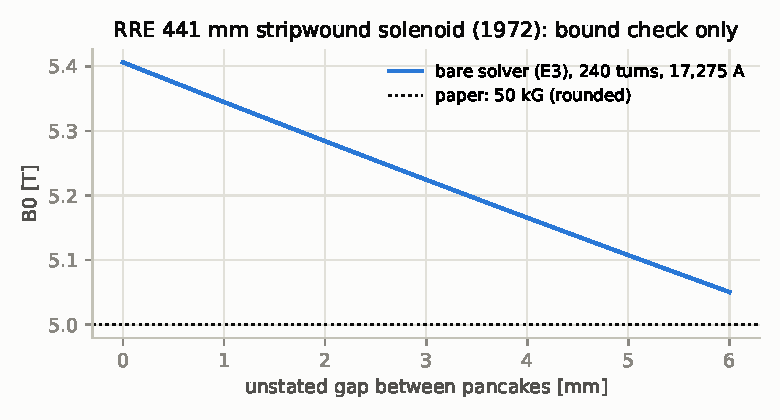
\includegraphics[width=0.62\textwidth]{fig18_rre_stripwound_bound}
\caption{RRE 441~mm stripwound solenoid: solver $B_0$ against the unstated inter-pancake gap.}
\label{fig:rre}
\end{figure}

\subsection{Consequences}
\begin{itemize}
\item Field is the only channel whose bare residual is small and smooth across geometries; it is the only one eligible for the residual corrector, which still needs a non-held-out campaign with a real validation split.
\item Inductance belongs in the physics model (PEEC), not in a corrector; measured $L$ is a target only with its frequency.
\item Resistance stays out of any corrector until voltage-tap positions and lead resistances are known.
\item Usable public data remains scarce: of the sources surveyed (\texttt{results/DATA\_SOURCES\_SURVEY.md}: arXiv, IEEE open copies, GitHub/Zenodo, theses, patents, facility pages), the NHMFL 41.5~T, HFML 38~T and UMBC 7~T magnets have measurements but no public coil tables, and the patents give design values only.
\end{itemize}

\FloatBarrier


\section{Interactive page}

\texttt{docs/index.html} (overview), \texttt{docs/demo.html} and \texttt{docs/bittersim.js} have no build step and no network requirement.
Sliders recompute the continuum model immediately.
Two presets fill the PDF initial guess and the seed-1 optimum at the geometry that prints 19.537~V, 17.974~kW, 21.153~C, 154.15~ppm and 4.543~V, 11.704~kW, 25.946~C, 99.95~ppm, 321.8~L/min.
A canvas draws the annulus, the plate pitch, the hole rows, a moving inlet-to-outlet marker, and the 30~mm DSV.
Copper colour is $J\propto 1/r$, or a cartoon temperature that is only a drawing.
A second canvas is a coarse elliptic-loop map of $B_z(\rho,z)$ with the DSV box and the printed ppm.
The emulation button draws quantile bars, a Langevin cloud, and an adiabatic sparkline that is captioned separately for the 4922~s optimum and the 479~s saturation path.
Out-of-catalog ids are refused.
Typed numbers outside the catalog window are clamped and the clamp is explained.

\section{How the report stays current}

\texttt{examples/run\_all.py} and \texttt{examples/run\_emulation.py} call \texttt{examples/update\_report.py}.
That script rewrites \texttt{report/generated\_numbers.tex} from \texttt{results/results.json} and \texttt{results/emulation\_compare.json}, then copies the report into \texttt{docs/} so the GitHub Pages tree can serve it.
It does not overwrite \texttt{results/results.json} with emulation output.
A later change of physics, of the page, or of a reported number is recorded with
\begin{verbatim}
python examples/update_report.py --append "what changed, tests, numbers"
\end{verbatim}
which appends \texttt{report/changelog.tex} and \texttt{PROJECT\_REPORT.md} in that same commit.
\texttt{python examples/update\_report.py --check} fails if the published printed figures or the Pages-demo changelog entry are missing.

\section{Generated numbers}
% Auto-generated by examples/update_report.py. Do not edit by hand.
\paragraph{Numerical tables regenerated 2026-10-02.}
\paragraph{Environment.} python 3.12.3, numpy 2.4.4, scipy 1.18.1, numba 0.68.0, matplotlib 3.11.2.
\begin{center}\begin{tabular}{lll}
\hline
quantity & PDF initial guess & seed-1 optimum \\
\hline
R1 [mm] & 50.00 & 50.01 \\
R2 [mm] & 150.00 & 300.00 \\
L [mm] & 800.0 & 1102.0 \\
current [A] & 920.0 & 2576.1 \\
voltage [V] & 19.537 & 4.543 \\
electrical power [kW] & 17.974 & 11.704 \\
hot-spot copper [C] & 21.153 & 25.946 \\
homogeneity [ppm] & 154.15 & 99.95 \\
flow [L/min] & 1834.9 & 321.8 \\
copper mass [kg] & 322 & 2575 \\
\hline
\end{tabular}\end{center}
Optimiser: differential\_evolution, 10605 evaluations, 125 s. Published pump-failure time to 85 C at the optimum is 4922 s. Hoop stress from the field profile is 0.1176 MPa. Heuristic Swiss-roll SNR gain is 4.745. Static permeability is 1.
\paragraph{Mesoscopic emulation, not molecular dynamics.}
Seed 1, 50 realizations. mesoscopic emulation, not molecular dynamics
\begin{center}\begin{tabular}{lrrrr}
\hline
quantity & nominal & p05 & p50 & p95 \\
\hline
B0 [T] & 0.500000 & 0.496394 & 0.500184 & 0.503441 \\
V [V] & 19.5366 & 19.3608 & 19.9514 & 20.4862 \\
P [W] & 17973.6 & 17811.8 & 18355.2 & 18847.2 \\
T hot [C] & 21.1528 & 21.0021 & 21.2889 & 21.5206 \\
ppm & 154.146 & 152.976 & 154.021 & 154.999 \\
drift [m/s] & 7.662703e-04 & 7.448405e-04 & 7.586380e-04 & 7.712947e-04 \\
mean free path [m] & 3.910825e-08 & 3.838720e-08 & 3.888908e-08 & 3.980924e-08 \\
Johnson [V] & 1.855013e-09 & 1.846957e-09 & 1.874151e-09 & 1.900141e-09 \\
\hline
\end{tabular}\end{center}
Trip fractions: hot spot above 85~C = 0.0, ONB margin below 0 = 0.0, stress above 0.6 yield = 0.0.
Adiabatic lumped trajectory. Interpretation stops at Tsat. The published time to 85 C is not a boiling model.
 PDF-guess adiabatic time to saturation in that file: 479.0 s.


\section{Changelog}
% Append-only. examples/update_report.py --append adds a paragraph.

\paragraph{2026-10-02, emulation layer.}
Separate catalog and mesoscopic emulation beside the continuum solver.
Python tests for that layer passed with the web-demo parity tests (16, then the full tree reached 47).
\texttt{examples/run\_all.py} reproduced the published seed-1 optimum.
Numbers in the published optimum table were not replaced.
The 50-draw, seed-1 emulation table is the PDF-guess comparison.

\paragraph{2026-10-02, Pages demo.}
Interactive \texttt{docs/index.html}: scaled plate drawing, coarse \(B_z\) map, presets, quantile bars, Langevin cloud, pump-failure sketch.
Report files are \texttt{PROJECT\_REPORT.md} and this LaTeX tree.
\texttt{examples/update\_report.py} rewrites \texttt{generated\_numbers.tex} whenever \texttt{run\_all.py} or \texttt{run\_emulation.py} finishes, and \texttt{--append} extends this changelog and \texttt{PROJECT\_REPORT.md}.
\paragraph{2026-10-02.}
Tests after the visual demo and the living report: 51 passed. Published continuum figures unchanged. PDF built locally from report/bitter\_solenoid\_report.tex (6 pages).

\paragraph{2026-10-07.}
Validation against measured magnets: Sabulsky Eq. 6 and Kobelev long-stack code checks; explicit layer stacks (bittersim/stack.py) with DC inductance and a PEEC AC-impedance model; bare-solver comparisons on EPFL (field -0.3 \%), Claw-ZS (field -1.1 \%, L(f) within 3 \% at 20 Hz-2 kHz, held out), JQI (shape within 0.1 \%, amplitude 9-12 \% high), Olsen (10 kHz |Z| miss +81 \% to +23 \%, held out) and a 1972 RRE bound; joint diagnostic shows one joint resistance does not generalize. Figures fig12-fig18. Nothing fitted. 133 tests pass.



\end{document}
